
% Uniswap V3 Neo4j-style graph reconstruction.
% Requires TikZ and xcolor.
% Scaling is handled by the parent figure environment.

\begingroup

% --------------------------------------------------
% Colors
% --------------------------------------------------

\definecolor{bloomEdge}{HTML}{64748B}
\definecolor{bloomInk}{HTML}{1E293B}
\definecolor{bloomDeployment}{HTML}{13C9C8}
\definecolor{bloomContract}{HTML}{E7C5E6}
\definecolor{bloomFunction}{HTML}{62C8CF}
\definecolor{bloomAction}{HTML}{A9D6F7}
\definecolor{bloomPool}{HTML}{C9B640}
\definecolor{bloomFamily}{HTML}{D4C08C}
\definecolor{bloomChain}{HTML}{A7D6F7}
\definecolor{bloomToken}{HTML}{1CD7B5}
\definecolor{bloomFee}{HTML}{7AE7A0}

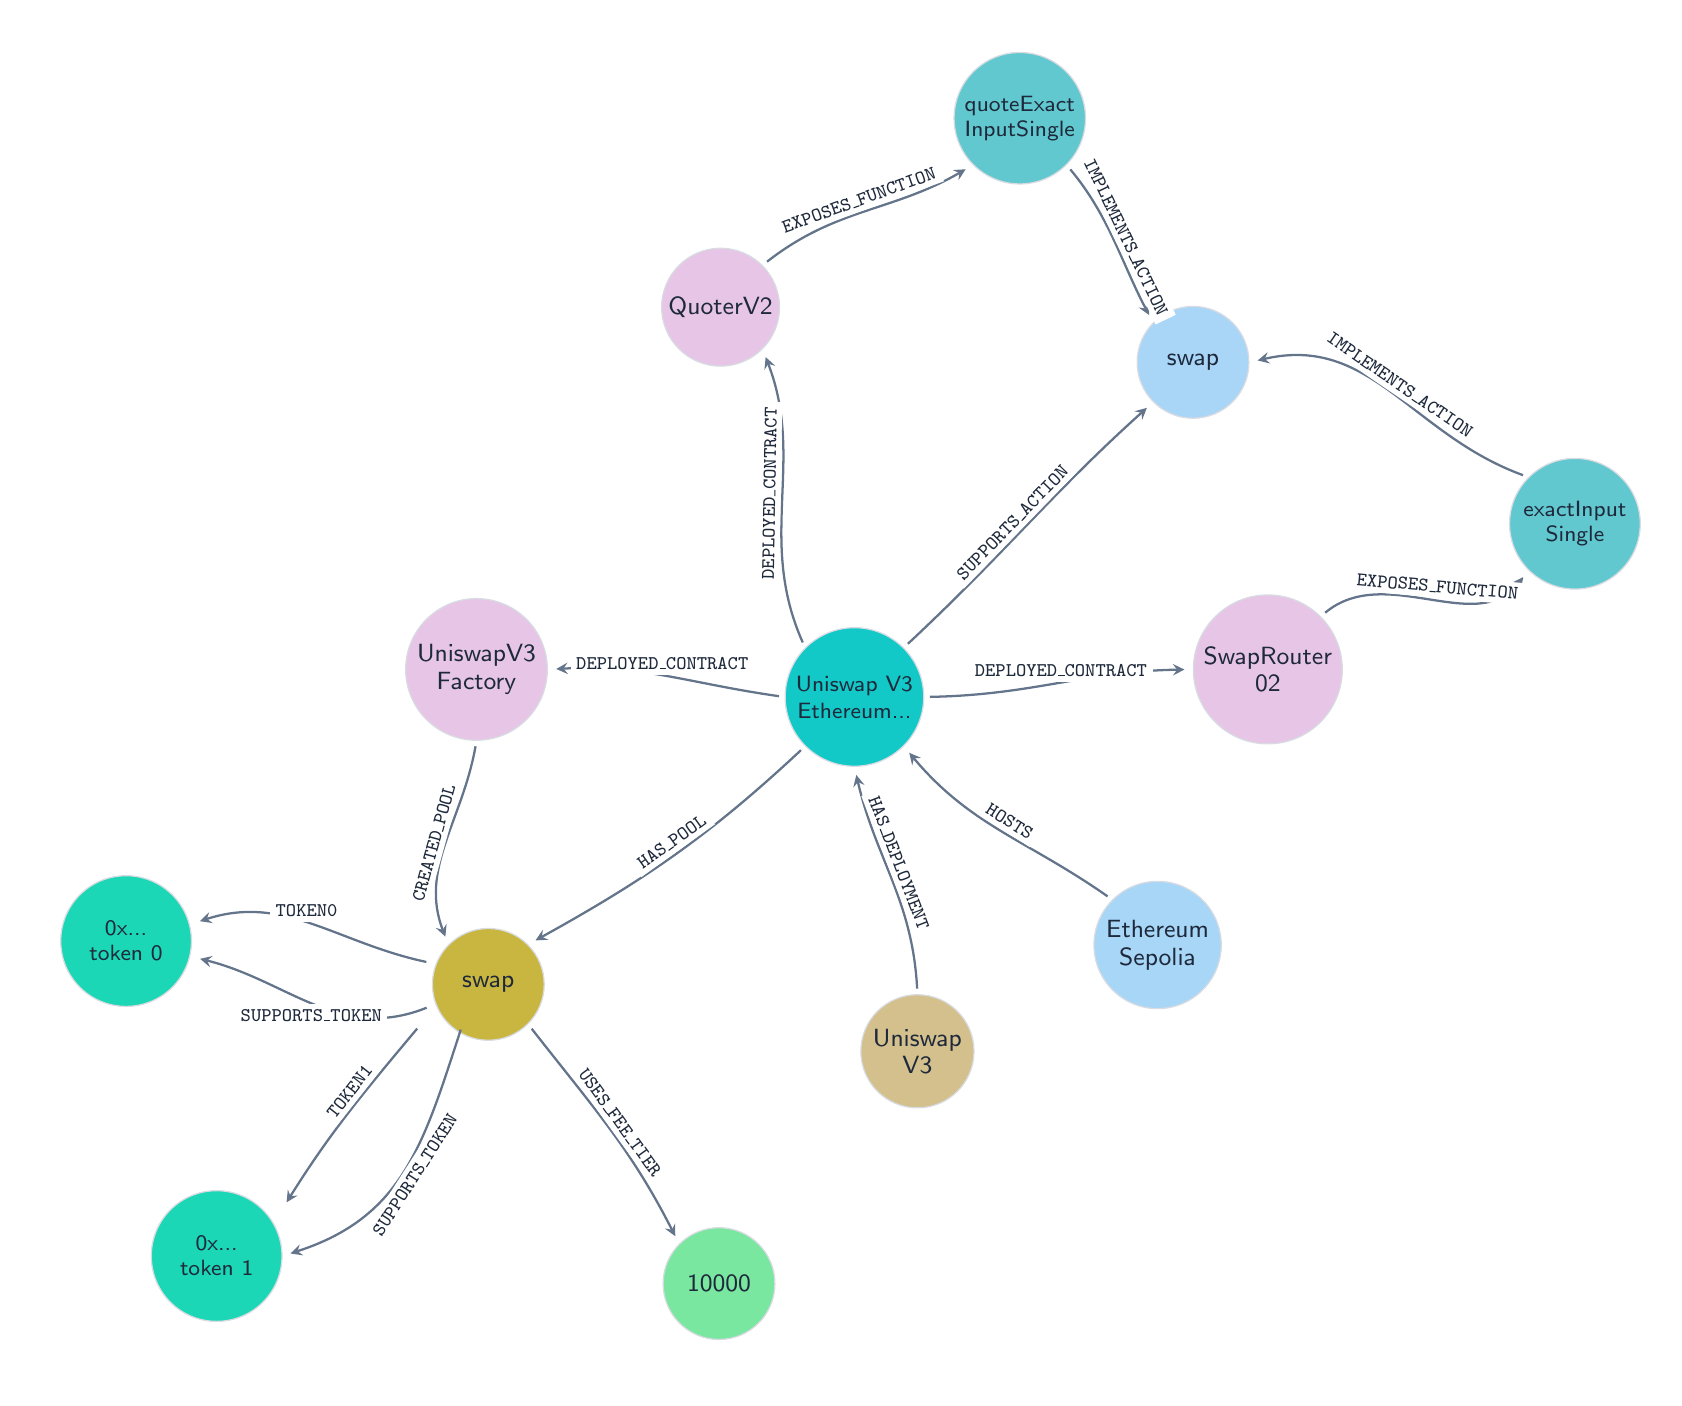
\begin{tikzpicture}[
  >=stealth,
  entity/.style={
    circle,
    draw=bloomEdge!25,
    line width=.45pt,
    fill=white,
    text=bloomInk,
    minimum size=1.42cm,
    inner sep=1.8pt,
    align=center,
    font=\sffamily\fontsize{8.8}{10}\selectfont
  },
  major/.style={
    entity,
    minimum size=1.76cm,
    font=\sffamily\fontsize{8.4}{9.8}\selectfont
  },
  longlabel/.style={
    entity,
    minimum size=1.66cm,
    font=\sffamily\fontsize{7.9}{9.0}\selectfont
  },
  link/.style={
    ->,
    draw=bloomEdge,
    line width=.82pt,
    shorten <=2pt,
    shorten >=3pt
  },
  relation/.style={
    fill=white,
    draw=none,
    text=bloomInk,
    inner xsep=2pt,
    inner ysep=1.9pt,
    font=\ttfamily\fontsize{7.1}{8.2}\selectfont
  }
]

% Consistent drawing boundary
\path[use as bounding box]
  (-10.5,-8.65) rectangle (10.15,8.5);

% --------------------------------------------------
% Graph entities
% --------------------------------------------------

\node[major,fill=bloomDeployment]
  (deployment) at (0,0)
  {Uniswap V3\\Ethereum...};

\node[entity,fill=bloomContract]
  (factory) at (-4.8,0.35)
  {UniswapV3\\Factory};

\node[entity,fill=bloomContract]
  (quoter) at (-1.7,4.95)
  {QuoterV2};

\node[longlabel,fill=bloomFunction]
  (quote) at (2.10,7.35)
  {quoteExact\\InputSingle};

\node[entity,fill=bloomAction]
  (action) at (4.3,4.25)
  {swap};

\node[entity,fill=bloomContract]
  (router) at (5.25,0.35)
  {SwapRouter\\02};

\node[longlabel,fill=bloomFunction]
  (execute) at (9.15,2.20)
  {exactInput\\Single};

\node[entity,fill=bloomChain]
  (chain) at (3.85,-3.15)
  {Ethereum\\Sepolia};

\node[entity,fill=bloomFamily]
  (family) at (0.80,-4.5)
  {Uniswap\\V3};

\node[entity,fill=bloomPool]
  (pool) at (-4.65,-3.65)
  {swap};

\node[longlabel,fill=bloomToken]
  (token0) at (-9.25,-3.1)
  {0x...\\token 0};

\node[longlabel,fill=bloomToken]
  (token1) at (-8.10,-7.1)
  {0x...\\token 1};

\node[entity,fill=bloomFee]
  (fee) at (-1.72,-7.45)
  {10000};

% --------------------------------------------------
% Protocol family and chain relationships
% --------------------------------------------------

% p1: ProtocolFamily -> ProtocolDeployment

\draw[link]
  (family.north)
  to[out=93,in=283,looseness=1.02]
  node[relation,sloped,above,pos=.56]
    {HAS\_DEPLOYMENT}
  (deployment.south);

% p2: Chain -> ProtocolDeployment

\draw[link]
  (chain.north west)
  to[out=145,in=310,looseness=1.03]
  node[relation,sloped,above,pos=.49]
    {HOSTS}
  (deployment.south east);

% --------------------------------------------------
% Deployment-to-contract relationships
% --------------------------------------------------

% p4: Deployment -> Factory

\draw[link]
  (deployment.west)
  to[out=172,in=3,looseness=1.02]
  node[relation,above,pos=.52]
    {DEPLOYED\_CONTRACT}
  (factory.east);

% p5: Deployment -> Quoter

\draw[link]
  (deployment.north west)
  to[out=114,in=291,looseness=1.01]
  node[relation,sloped,above,pos=.52]
    {DEPLOYED\_CONTRACT}
  (quoter.south east);

% p3: Deployment -> SwapRouter

\draw[link]
  (deployment.east)
  to[out=1,in=181,looseness=1.03]
  node[relation,above,pos=.51]
    {DEPLOYED\_CONTRACT}
  (router.west);

% --------------------------------------------------
% Quoter and preflight function
% --------------------------------------------------

% Quoter -> quoteExactInputSingle

\draw[link]
  (quoter.north east)
  to[out=38,in=210,looseness=1.03]
  node[relation,sloped,above,pos=.49]
    {EXPOSES\_FUNCTION}
  (quote.south west);

% quoteExactInputSingle -> swap action

\draw[link]
  (quote.south east)
  to[out=-50,in=118,looseness=.94]
  node[relation,sloped,above,pos=.51]
    {IMPLEMENTS\_ACTION}
  (action.north west);

% --------------------------------------------------
% Router and execution function
% --------------------------------------------------

% SwapRouter -> exactInputSingle

\draw[link]
  (router.north east)
  to[out=40,in=233,looseness=1.01]
  node[relation,sloped,above,pos=.53]
    {EXPOSES\_FUNCTION}
  (execute.south west);

% exactInputSingle -> swap action

\draw[link]
  (execute.north west)
  to[out=160,in=13,looseness=1.06]
  node[relation,sloped,above,pos=.49]
    {IMPLEMENTS\_ACTION}
  (action.east);

% --------------------------------------------------
% Deployment supports swap
% --------------------------------------------------

\draw[link]
  (deployment.north east)
  to[out=43,in=222,looseness=1.01]
  node[relation,sloped,above,pos=.47]
    {SUPPORTS\_ACTION}
  (action.south west);

% --------------------------------------------------
% Factory and pool relationships
% --------------------------------------------------

% Factory -> Pool

\draw[link]
  (factory.south)
  to[out=260,in=111,looseness=1.01]
  node[relation,sloped,above,pos=.51]
    {CREATED\_POOL}
  (pool.north west);

% Deployment -> Pool

\draw[link]
  (deployment.south west)
  to[out=223,in=29,looseness=1.0]
  node[relation,sloped,above,pos=.48]
    {HAS\_POOL}
  (pool.north east);

% --------------------------------------------------
% Pool -> Token 0
% Separate curved lanes
% --------------------------------------------------

% p8: TOKEN0

\draw[link]
  ([yshift=2.7mm]pool.west)
  to[out=168,in=18,looseness=1.02]
  node[relation,above,pos=.52]
    {TOKEN0}
  ([yshift=2.2mm]token0.east);

% p10: SUPPORTS_TOKEN

\draw[link]
  ([yshift=-2.7mm]pool.west)
  to[out=202,in=-14,looseness=1.03]
  node[relation,below,pos=.51]
    {SUPPORTS\_TOKEN}
  ([yshift=-2.0mm]token0.east);

% --------------------------------------------------
% Pool -> Token 1
% Independently curved relationship paths
% --------------------------------------------------

% p9: TOKEN1

\draw[link]
  ([xshift=-3.5mm]pool.south west)
  to[out=230,in=58,looseness=1.0]
  node[relation,sloped,above,pos=.41]
    {TOKEN1}
  ([xshift=2.4mm]token1.north east);

% p11: SUPPORTS_TOKEN

\draw[link]
  ([xshift=1.8mm]pool.south west)
  to[out=252,in=18,looseness=1.10]
  node[relation,sloped,below,pos=.49]
    {SUPPORTS\_TOKEN}
  (token1.east);

% --------------------------------------------------
% Pool -> FeeTier
% --------------------------------------------------

% p12: USES_FEE_TIER

\draw[link]
  (pool.south east)
  to[out=-52,in=117,looseness=1.03]
  node[relation,sloped,above,pos=.50]
    {USES\_FEE\_TIER}
  (fee.north west);

\end{tikzpicture}
\endgroup
